\chapter{Methodology}\label{chapter:methodology}
In this section, the established infrastructure required for measuring and monitoring the power consumption of the various employed edge devices will be introduced. Moreover, the chosen approach to distribute the power consumption of an edge device among the individual function executions will be explained.

\section{Establishment of the Edge Cluster}
The experimental cluster that served as the foundation of this work was set up using \textit{k3s}, which is a lightweight distribution of Kubernetes primarily designed for edge computing and IoT applications. Due to its compatibility with ARMv7- and ARM64-based devices it offers the possibility to establish a Kubernetes cluster composed of heterogeneous edge computers and is thus perfectly suitable for the purpose of this work. Additionally, k3s does not place great demands on the hardware equipment which is why it can be deployed to a wide range of different devices, even to those with strictly limited resources~\parencite{k3s}.\\
After installing Docker on the employed edge computers, each device was added to the cluster by running the k3s agent using the corresponding token required to perform a join. The inidividual nodes of the resulting cluster as well as the role that they fulfill are outlined by Table \ref{table:1}.

\begin{center}
\begin{table}[h!]
\centering
\begin{tabular}{||c c||} 
 \hline
 Node & Cluster Role \\ [0.5ex] 
 \hline\hline
 Linux Virtual Machine & Master \\ 
 \hline
 Raspberry Pi 3 Model B v1.2 & Worker \\ 
 \hline
 PYNQ-Z1 & Worker \\
 \hline
 ODROID-XU4 & Worker \\
 \hline
 ODROID-XU4 Shifter Shield & Worker \\
 \hline
 Google Coral Dev Board & Worker \\
 \hline
 NVIDIA Jetson Nano & Worker \\ [1ex] 
 \hline
\end{tabular}
\caption{Topology of the experimental Kubernetes Edge-Cluster.}
\label{table:1}
\end{table}
\end{center}

\section{Implementation of the Power Consumption Measurements}
Measuring the energy consumption of an electronic device is not a trivial task due to the fact that software solutions are very limited in their functionality and thus only allow for an estimation rather than an accurate measurement. Therefore, a hardware-based approach was chosen in this work in order to get more meaningful and precise data regarding the power consumption of the employed single-board computers. To this end, the power measurements are carried out by a powermeter developed at the Technical University of Munich, which consists of an ESP32 micro-controller that is connected with two INA3221 sensors via I$^{2}$C, which is a short-distance, on-board communication protocol based on the master-slave architecture. The following two sections aim on giving a more detailed overview of these components.

\subsection{ESP32 Powermeter}

\subsubsection{ESP32 (ESP32-WROOM-32E)}
The ESP32 is a family of micro-controllers manufactured by the chinese company Espressif, which integrates perfectly with IoT applications due to the fact that each model has integrated support for WiFi and Bluetooth and is shipped with a multitude of different peripheral interfaces (e.g. for I$^{2}$C) that can be used to connect sensors, displays or cameras. The concrete module that was employed for this work is the ESP32-WROOM-32E, which is equipped with a 32-bit Xtensa LX6 Dual-Core microprocessor that operates at up to 240 MHz. Moreover, it is provided with 448 KB of ROM and 520 KB of SRAM and requires a power supply of around 3V - 3.6V. Figure 3.1 shows the ESP32-WROOM-32E module integrated into a development board.\\
The ESP32 chip is especially suitable for applications where energy consumption is crucial since it has a sleep current of less than 5 µA and offers the possibility to lower the CPU clock frequency down to 80 MHz. Additionally, it has access to a low-power coprocessor that can be used instead of the CPU to perform tasks that don't require much computational power~\parencite{esp32-manual}.\\
In order to facilitate software development for the ESP32, Espressif offers the \textit{Espressif IoT Development Framework} (ESP-IDF) which can be used to build and flash software onto an arbitrary ESP32 board. ESP-IDF can either be installed manually or integrated into the well-known Integrated Development Environments (IDEs) Visual Studio Code and Eclipse.

\begin{figure}[h]
    \centering
    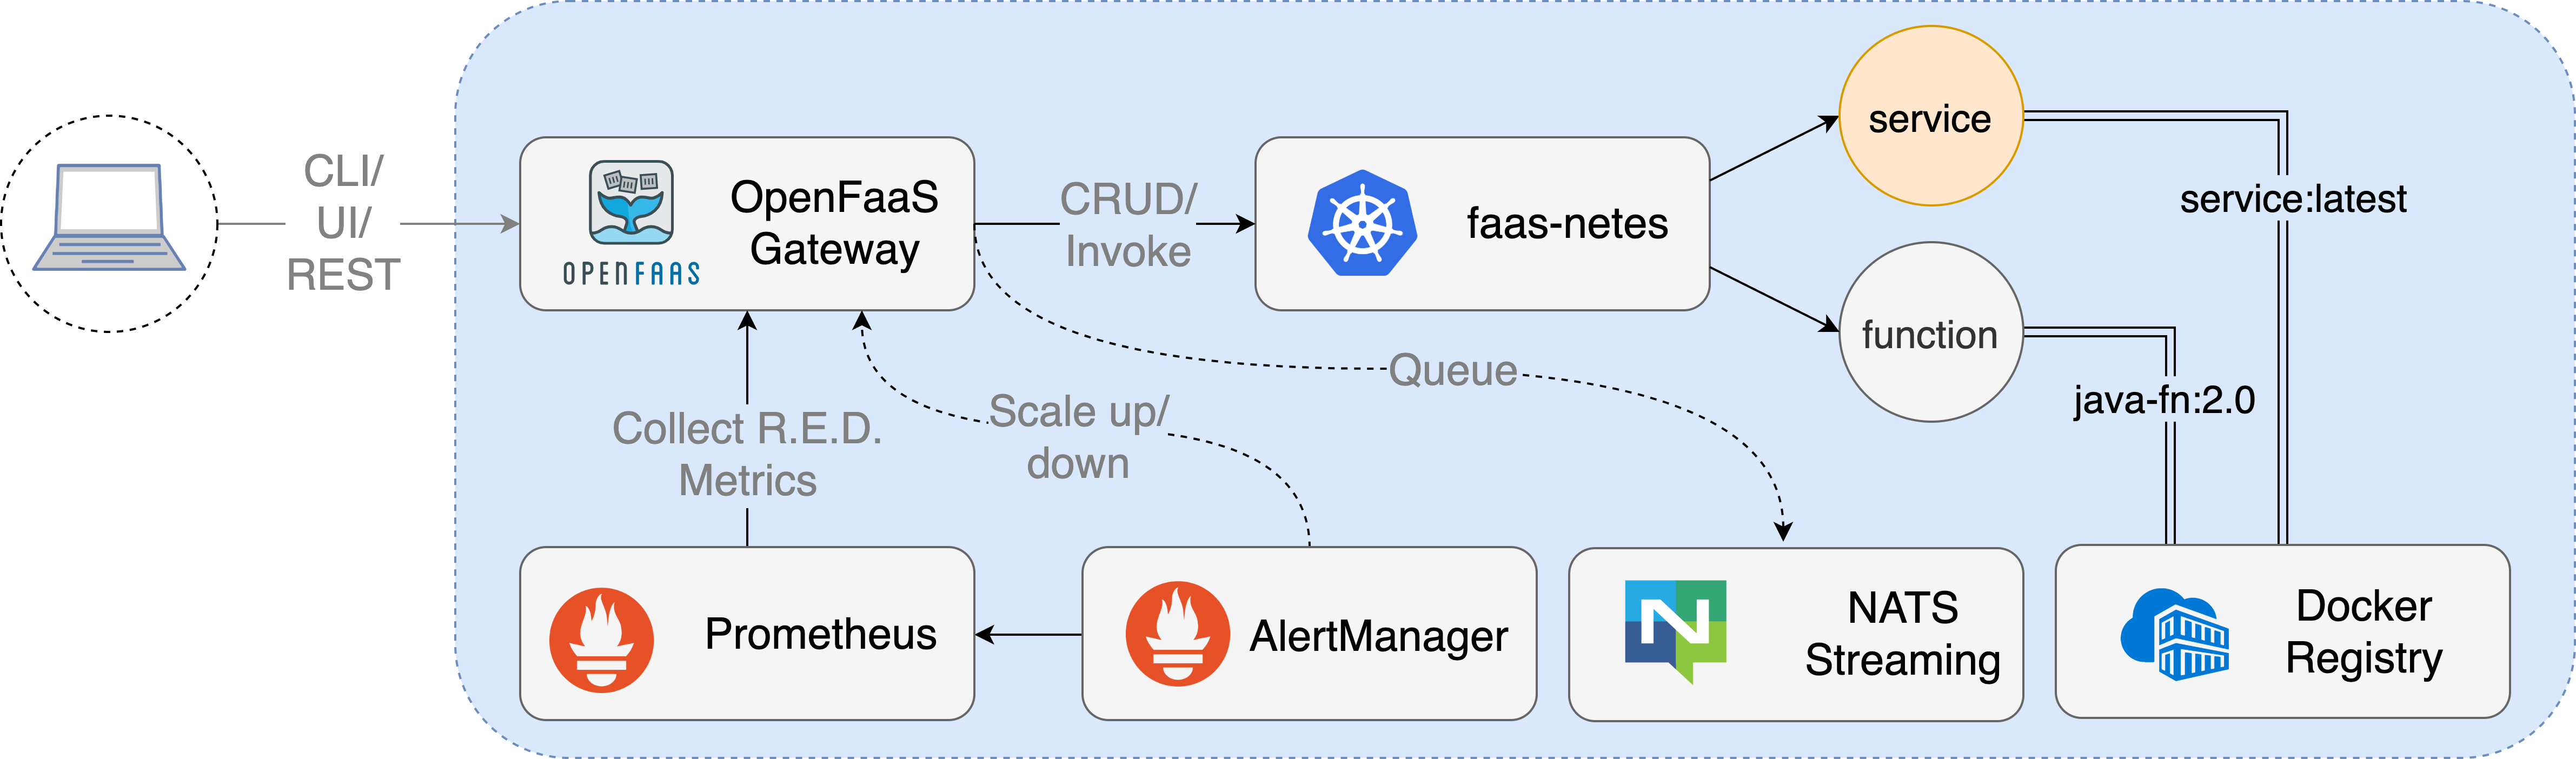
\includegraphics[width=1\textwidth]{./figures/of-workflow.png}
    \caption{Interaction with the OpenFaaS API Gateway~\parencite{openfaas-stack}}
    \label{fig:openfaas-gateway}
\end{figure}

\subsubsection{INA3221}
The INA3221 is a triple-channel sensor platform manufactured by Texas Instruments, which is designed to accurately measure and monitor both current and voltage for up to three unique power-supply rails. The buses monitored by the sensor can range from 0V at the minimum and 26V at the maximum, while the INA3221 itself draws a supply current of around 350 µA and requires a power supply that ranges between 2.7V - 5.5V in order to be operated~\parencite{ina3221-manual}. For communication with external devices it is provided with an I$^{2}$C- and SMBUS-compatible interface that allows for four different programmable addresses GND, SCL, SDA and $V_{S}$ which are controlled by the single address pin A0.\\
The INA3221 uses a so-called shunt resistor at every channel in order to measure the current flowing through the shunt by measuring the generated voltage drop across the resistor. Since the resistance is known, Ohm's Law can be applied in order to calculate the current.\\

\begin{equation}
   Current (A) = \frac{Voltage (V)}{Resistance (R)}
\end{equation}

\subsection{Interfacing the Powermeter via WiFi}


\section{Integration of Power Consumption Monitoring}
In order to integrate the energy consumption measurements of the individual edge systems into the existing monitoring infrastructure ...

\section{Inference of Power Consumption to Function Executions}